%                            ================================
%                            [Type doctument]
%                            - \documentclass[option]{class}
%                            [Other page setup]
%                            - geometry: set margin, should
%                                similar with \documentclass
%                            ================================
\documentclass[12pt, a4paper, twoside]{report}
\usepackage[a4paper,inner=3cm,outer=2cm]{geometry}

%============================================================
% Preamble
% - Include packages allow expand ability of Texlive by more 
%       commands, environments
% - Commands effect entire document
%============================================================
%                            ================================
%                            Package
%                            - lipsum: lorem paragraph
%                            Url
%                            - hyperref: url
%                            Color
%                            - color, xcolor
%                            Language format
%                            - inputenc, fontenc, babel
%                            - lmodern: Latin modern
%                            Table
%                            - array: format tabular row
%                            - graphicx: table size
%                            Render basic
%                            - rotating: rotate object 
%                                       (static or float)
%                            - rotfloat: addition float rotating
%                            - float: addition H absolute position
%                               for rotfloat or table, figure evironment
%                            - graphicx: image like PNG, IMG, PDF
%                            ================================
\usepackage{lipsum}
\usepackage[hidelinks]{hyperref}
% \usepackage{color}
\usepackage[table]{xcolor}

\usepackage[utf8]{inputenc}
\usepackage[T5,T1]{fontenc}
\usepackage{lmodern} % a Latin font version enhance from
                        % cm-supper + vector format + better support T1,T5
\usepackage[vietnamese, english]{babel} 


\usepackage{array}
\usepackage{graphicx}


\usepackage{rotating}
\usepackage{rotfloat}

\usepackage{float}

\usepackage{graphicx}

%============================================================
% Document
% - Plain text, list of tables, figures, input other tex, 
%       bibilography, ...
% - Commands with scope: in group
% - Environments differ from 'document': 
%       /begin{env} , /end{env}
%============================================================
\begin{document}
%                                                        ================================
%                                                        [Front matter]
%                                                        2. Empty
%                                                        3. Title page
%                                                        4. Information (copyright notice, ISBN, etc.)
%                                                        5. Dedication if any, else empty
%                                                        6. Table of contents
%                                                        7. List of figures (can be in the backmatter too)
%                                                        8. Preface chapter
%                                                        ================================


%                            ================================
%                            Title
%                            ================================
\title{\textbf{Hello\thanks{\LaTeX {} wikibook}}}
\author{Giang Trinh\thanks{GitHub: \url{{https://github.com/TrinhHuuGiang}}}
    \and others\thanks{No one}}
\maketitle
%                            ================================
%                            Abstract
%                            ================================

%                            ================================
%                            Table of contents
%                            - TOC, LOF, LOT
%                            ================================
\tableofcontents
\listoftables
\listoffigures


%                                                        ================================
%                                                        [Main matter]
%                                                        - Main topics
%                                                        ================================
\chapter{This is test chapter}
\section{This is numbering section 1}

\section*{This is unnumbering section, hiden from TOC}
\section{This is numbering section 2}

\phantomsection
\addcontentsline{toc}{section}{This is title of unnumbering, sometime use for Openning, Preface}
\section*{This is unnumbering section, show in TOC by phantomsectom, addcontentline}

\section{This is numbering section 3}

\section[This is short of section 4]{This is section 4}



% rotating
\chapter{This is float environment example}

% \begin{sideways}
\begin{sideways}
    \parbox{10cm}
    {
        \lipsum[1]\\
        
        \lipsum[2]
    }

    \parbox{10cm}
    {
        \lipsum[2]
    }

\end{sideways}


% \begin{turn}{counter clock angle}
\newpage

\begin{turn}{45}
    \parbox{10cm}
    {
        \lipsum[1]\\
        
        \lipsum[2]
    }

    \parbox{10cm}
    {
        \lipsum[2]
    }

\end{turn}



% Table environment / sidewaystable environment
\newpage
\rowcolors{1}{lightgray}{yellow}
\setlength{\arrayrulewidth}{1pt}

\begin{sidewaystable}[htbp]

    \raggedleft

    \caption{This is template table 1, caption top}

    \begin{turn}{30}
        \begin{tabular}{|c|}
            
            \hline

            \parbox{10cm}
            {
                \hspace{0pt} \\
                \lipsum[1] \\
            } \\

            \hline

            \parbox{10cm}
            {
                \hspace{0pt} \\
                \lipsum[2] \\
            } \\

            \hline

        \end{tabular}
    \end{turn}

    \caption{This is template table 1, caption bottom}

\end{sidewaystable}

\textbf{\textcolor{red}{
    Float table should be here but go `page for floats' because there is no space
    }
} \\

\lipsum[1]\\
\lipsum[1]\\
\lipsum[1]\\

% rendering image

\newpage
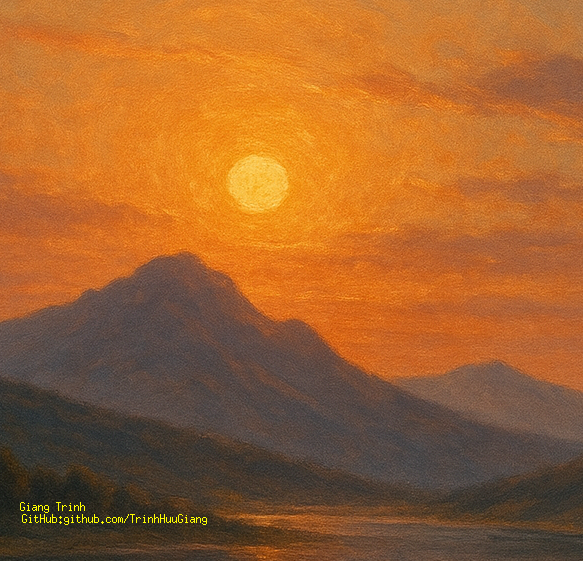
\includegraphics[width=5cm, keepaspectratio=true, angle=20]{./sunset.png} This is image width 5cm\\

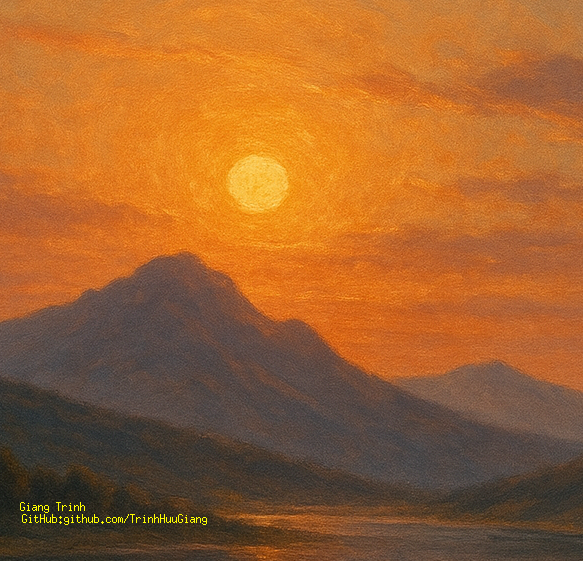
\includegraphics[width=5cm, keepaspectratio=true, angle=20, scale=0.5]{./sunset.png} Scale factor 0.5\\

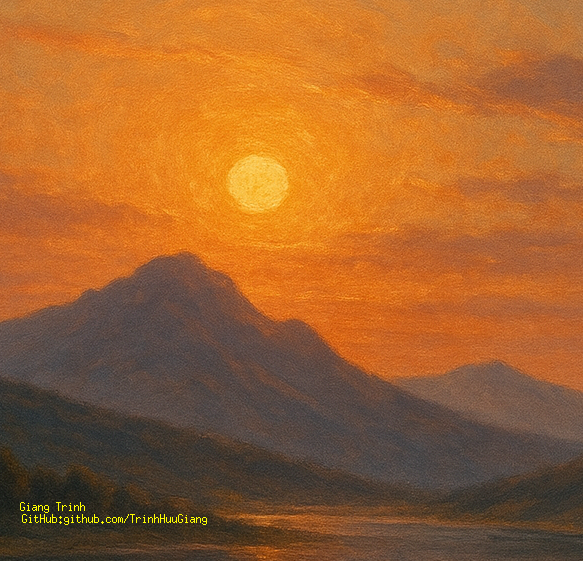
\includegraphics[width=5cm, keepaspectratio=true, angle=20, scale=1.5]{./sunset.png} Scale factor 1.5\\



%                                                        ================================
%                                                        Appendix
%                                                        - Subordinate chapters
%                                                        ================================

%                                                        ================================
%                                                        Back matter
%                                                        - Bibliography
%                                                        - Glossary/Index
%                                                        ================================





%                            ================================
%                            END
%                            ================================
\end{document}

